\documentclass[11pt,a4paper]{article}
\usepackage[etiket=en]{gtu-el-yazisi}
% üstü çizili (sadeleşen) terim
\newcommand\sil[1]{\tikz[baseline=(s.base)]{\node[inner sep=0.6pt](s){$#1$};\draw[line width=0.5pt](s.south west)--(s.north east);}}
\newcommand\parantez[1]{$\left.\vrule height #1 depth #1 width 0pt\right\}$}
\begin{document}
\notbilgi{Elektronik I}{Final notu -- BJT ve MOSFET özeti, küçük işaret modelleri}{Final-notu.pdf}

\sayfa{1}
\section{BJT}
\noindent
\begin{minipage}[c]{0.3\linewidth}
\centering
\begin{circuitikz}[line width=0.6pt, color=kirmizikalem]
  \draw (0,0) node[npn](Q){};
  \draw (Q.B) node[left]{B};
  \draw (Q.C) node[right]{C};
  \draw (Q.E) node[right]{E\ \ $n$};
  \node[below left] at (Q.E) {npn\quad};
\end{circuitikz}
\end{minipage}\hfill
\begin{minipage}[c]{0.68\linewidth}
\[ i_C = I_S\, e^{v_{BE}/V_T} \]
\[ \kutula{i_B = \frac{i_C}{\beta}} \qquad \kutula{i_E = \frac{\beta+1}{\beta}\, i_C} = \frac{1}{\alpha}\, i_C \]
\[ \kutula{i_E = (\beta+1)\, i_B} \]
\end{minipage}

\begin{center}
\begin{tabular}{llll}
  \toprule
      & Active & Sat & Cutoff \\ \midrule
  EBJ & \textcolor{kirmizikalem}{Forward bias} & \textcolor{kirmizikalem}{Forward bias} & \textcolor{kirmizikalem}{Reverse bias} \\
  CBJ & \textcolor{kirmizikalem}{Reverse bias} & \textcolor{kirmizikalem}{Forward bias} & \textcolor{kirmizikalem}{Reverse bias} \\ \bottomrule
\end{tabular}
\end{center}

\noindent
\begin{minipage}[t]{0.49\linewidth}
\underline{In npn}

\centering
\begin{circuitikz}[line width=0.6pt]
  \draw (0,0) node[left]{$p$\ \ B} to[short, o-*] (0.7,0);
  \draw (0.7,0) |- (1.2,0.9) to[D] (2.8,0.9) to[short, -o] (3.2,0.9) node[right]{C\ \ $n$};
  \draw (0.7,0) |- (1.2,-0.9) to[D] (2.8,-0.9) to[short, -o] (3.2,-0.9) node[right]{E\ \ $n$};
\end{circuitikz}

\raggedright
\underline{Active}: $V_{BE} \geqslant 0{,}7,\ V_{BC} \leqslant 0{,}4\,\mathrm{V}$

\underline{Cutoff}: $V_{BE} < 0{,}7,\ V_{BC} \leqslant 0{,}4\,\mathrm{V}$

\underline{Saturation}: $V_{BE} \geqslant 0{,}7,\ V_{BC} > 0{,}4\,\mathrm{V}$
\end{minipage}\hfill
\begin{minipage}[t]{0.49\linewidth}
\underline{In pnp}

\centering
\begin{circuitikz}[line width=0.6pt]
  \draw (0,0) node[pnp](P){};
  \draw (P.B) node[left]{B\ \ $n$};
  \draw (P.E) node[right]{E\ \ $p$};
  \draw (P.C) node[right]{C\ \ $p$};
\end{circuitikz}

\raggedright
\underline{Active}: $V_{EB} \geqslant 0{,}7,\ V_{CB} \leqslant 0{,}4\,\mathrm{V}$

\underline{Cutoff}: $V_{EB} < 0{,}7,\ V_{CB} \leqslant 0{,}4\,\mathrm{V}$

\underline{Saturation}: $V_{EB} \geqslant 0{,}7\,\mathrm{V},\ V_{CB} > 0{,}4\,\mathrm{V}$
\end{minipage}

\subsection{Small signal Models}
\noindent
\begin{minipage}[c]{0.16\linewidth}
\centering
\begin{circuitikz}[line width=0.6pt]
  \draw (0,0) node[npn](Q){};
  \draw (Q.B) node[left]{B};
  \draw (Q.C) node[right]{C};
  \draw (Q.E) node[right]{E};
\end{circuitikz}
\end{minipage}\hfill
\begin{minipage}[c]{0.56\linewidth}
\centering
\begin{circuitikz}[line width=0.6pt]
  \draw[dashed, morkalem] (0.35,-0.45) rectangle (6.45,2.85);
  \draw (0,2) node[left]{B} to[short, *-, i>^=$i_b$] (1.5,2) to[R, l=$r_\pi$] (1.5,0) -- (5.6,0);
  \node at (1.1,1.55) {$+$}; \node at (1.0,1.0) {$v_\pi$}; \node at (1.1,0.45) {$-$};
  \draw (3.8,2) to[cisource, l=$g_m v_\pi$] (3.8,0);
  \draw (3.8,2) -- (5.6,2) to[R, l=$r_o$] (5.6,0);
  \draw (5.6,2) to[short, -*, i<^=$i_c$] (7,2) node[right]{C};
  \draw (3,0) to[short, -o] (3,-0.9) node[below]{E\ \ $\downarrow i_e$};
\end{circuitikz}
\end{minipage}\hfill
\begin{minipage}[c]{0.24\linewidth}
\formulkutu{i_b = \dfrac{v_\pi}{r_\pi}}
\end{minipage}

\medskip
$r_o \rightarrow$ output resistance of bjt : $r_o = \dfrac{|V_A|}{I_C}$ \quad ($I_C \rightarrow$ DC)

\medskip
$g_m \rightarrow$ transcunductance : $g_m = \dfrac{I_C}{V_T}$

\medskip
$r_\pi \rightarrow$ base resistance : $r_\pi = (\beta+1)\, r_e$

\medskip
$r_e \rightarrow$ emitter resistance : $r_e = \dfrac{V_T}{I_E} = \alpha\,\dfrac{V_T}{I_C} = \overset{1}{\sil{\alpha}}\,\dfrac{1}{g_m}$

\subsection{T model}
\noindent
\begin{minipage}[c]{0.5\linewidth}
\centering
\begin{circuitikz}[line width=0.6pt]
  \draw (0,4) -- (3,4) to[short, -*] (4,4) node[right]{C};
  \draw (0,4) to[cisource, l=$\alpha i_e / g_m V_\pi$] (0,2);
  \draw (-1.3,2) node[left]{B} to[short, *-*] (0,2);
  \draw (0,2) to[R, l=$r_e$, i>^=$i_e$] (0,0) -- (3,0);
  \draw (3,4) to[R, l=$r_o$] (3,0);
  \draw (1.5,0) to[short, *-*] (1.5,-0.8) node[below]{E};
  \node at (-0.4,1.6) {$+$}; \node at (-0.65,1.0) {$V_\pi$}; \node at (-0.4,0.4) {$-$};
\end{circuitikz}
\end{minipage}\hfill
\begin{minipage}[c]{0.48\linewidth}
\begin{align*}
  r_o &= \frac{|V_A|}{I_C} \\
  g_m &= \frac{I_C}{V_T} \\
  r_\pi &= (\beta+1)\, r_e \\
  r_e &= \frac{V_T}{I_E} = \alpha\, \frac{V_T}{I_C} = \overset{1}{\sil{\alpha}}\, \frac{1}{g_m}
\end{align*}
\end{minipage}

\bigskip
\noindent
\begin{minipage}[c]{0.56\linewidth}
\centering
\begin{circuitikz}[line width=0.6pt]
  \draw (0,0) rectangle (2.6,1.8);
  \node at (1.3,0.9) {Circuit};
  \draw (-1.2,1.4) to[short, o-] (0,1.4);
  \draw (-1.2,0.4) to[short, o-] (0,0.4);
  \draw (2.6,1.4) to[short, -o] (3.8,1.4);
  \draw (2.6,0.4) to[short, -o] (3.8,0.4);
  \node at (-1.1,1.15) {\small$+$}; \node at (-0.75,0.9) {$v_i$}; \node at (-1.1,0.62) {\small$-$};
  \node at (4.0,1.4) {\small$+$}; \node at (4.15,0.9) {$v_o$}; \node at (4.0,0.4) {\small$-$};
  \draw[-{Latex[length=2mm]}] (-1.6,-0.5) -- (-1.6,0.9) -- (-1.1,0.9);
  \node[below] at (-1.6,-0.5) {$R_{in}$};
  \draw[-{Latex[length=2mm]}] (3.2,-0.5) -- (3.2,0.9) -- (2.8,0.9);
  \node[below] at (3.2,-0.5) {$R_{out}$};
\end{circuitikz}
\end{minipage}\hfill
\begin{minipage}[c]{0.42\linewidth}
\underline{Voltage Gain}

$A_v = \dfrac{v_o}{v_i}$

$R_{in} \rightarrow$ Input Resistance

$R_{out} \rightarrow$ Output Res.
\end{minipage}

\clearpage
\section{Mosfet}
\subsection{NMOS}
\noindent
\begin{minipage}[c]{0.22\linewidth}
\centering
\begin{circuitikz}[line width=0.6pt]
  \draw (0,0) node[nmos, arrowmos](M){};
  \draw (M.G) node[left]{G};
  \draw (M.D) node[right]{D};
  \draw (M.S) node[right]{S};
\end{circuitikz}
\end{minipage}\hfill
\begin{minipage}[c]{0.76\linewidth}
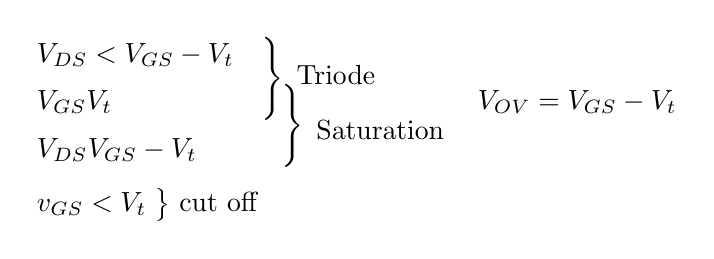
\begin{tikzpicture}
  \node[anchor=west] at (0,1.2) {$V_{DS} < V_{GS} - V_t$};
  \node[anchor=west] at (0,0.6) {$V_{GS} \geqslant V_t$};
  \node[anchor=west] at (0,0) {$V_{DS} \geqslant V_{GS} - V_t$};
  \node at (3.1,0.9) {\parantez{4.5mm}};
  \node[anchor=west] at (3.3,0.95) {Triode};
  \node at (3.35,0.3) {\parantez{4.5mm}};
  \node[anchor=west] at (3.55,0.25) {Saturation};
  \node[anchor=west] at (5.6,0.6) {$V_{OV} = V_{GS} - V_t$};
  \node[anchor=west] at (0,-0.7) {$v_{GS} < V_t \;\bigr\}$ cut off};
\end{tikzpicture}
\end{minipage}

\begin{center}
\begin{tikzpicture}
  \node (n) at (0,0) {NMOS};
  \draw (n.south) -- (0,-0.55);
  \draw[-{Latex[length=2mm]}] (0,-0.55) -- (-3.9,-0.55) -- (-3.9,-0.9);
  \draw[-{Latex[length=2mm]}] (0,-0.55) -- (3.9,-0.55) -- (3.9,-0.9);
  \node at (-3.9,-1.2) {Triode};
  \node at (0,-1.1) {$v_{GS} \geqslant V_t$};
  \node[align=center] at (3.9,-1.35) {Saturation\\[-1mm] Region};
  \node at (-3.9,-2.1) {$V_{GD} > V_t$};
  \node at (3.9,-2.1) {$V_{GD} \leqslant V_t$};
  \node at (-3.9,-2.8) {$V_{DS} < V_{OV}$};
  \node at (3.9,-2.8) {$V_{DS} \geqslant V_{OV}$};
  \node[anchor=north] at (-3.9,-3.25) {$i_D = \underset{\substack{\swarrow\\ \mu_n C_{ox}}}{k_n'} \left(\dfrac{W}{L}\right) \left(V_{OV} - \dfrac{1}{2} V_{DS}\right) V_{DS}$};
  \node[anchor=north] at (3.9,-3.25) {$i_D = \dfrac{1}{2}\, k_n' \left(\dfrac{W}{L}\right) v_{OV}^2$};
\end{tikzpicture}
\end{center}

\subsection{PMOS}
\begin{center}
\begin{tikzpicture}
  \node (p) at (0,0) {PMOS};
  \draw (p.south) -- (0,-0.55);
  \draw[-{Latex[length=2mm]}] (0,-0.55) -- (-3.9,-0.55) -- (-3.9,-0.9);
  \draw[-{Latex[length=2mm]}] (0,-0.55) -- (3.9,-0.55) -- (3.9,-0.9);
  \node at (-3.9,-1.2) {Triode Region};
  \node at (3.9,-1.2) {Saturation Region};
  \node at (-3.9,-1.9) {$V_{DG} > |V_t|$};
  \node at (3.9,-1.9) {$V_{DG} \leqslant |V_t|$};
  \node at (-3.9,-2.6) {$V_{SD} < |V_{OV}|$};
  \node at (3.9,-2.6) {$V_{SD} \geqslant |V_{OV}|$};
  \node[anchor=north] at (-3.9,-3.05) {$i_D = k_p' \left(\dfrac{W}{L}\right) \left(|V_{OV}| - \dfrac{1}{2} V_{SD}\right) V_{SD}$};
  \node[anchor=north] at (3.9,-3.05) {$i_D = \dfrac{1}{2}\, k_p' \left(\dfrac{W}{L}\right) V_{OV}^2$};
\end{tikzpicture}
\end{center}

\subsection{Mosfet small signal}
\subsubsection{\texorpdfstring{$\pi$}{pi} model}
\begin{center}
\begin{circuitikz}[line width=0.6pt]
  \draw (0,2) node[left]{G} to[short, *-] (1.4,2) to[short, -o] (1.4,1.6);
  \draw (1.4,0.8) to[short, o-] (1.4,0.4) -- (5,0.4);
  \node at (1.05,1.5) {\small$+$}; \node at (0.8,1.2) {$v_{gs}$}; \node at (1.05,0.9) {\small$-$};
  \draw (3,2) to[cisource, l=$g_m V_{gs}$] (3,0.4);
  \draw (3,2) -- (5,2) to[R, l=$r_o$] (5,0.4);
  \draw (5,2) to[short, -o, i<^=$I_D$] (6,2) node[right]{D};
  \draw (2.2,0.4) to[short, -o] (2.2,-0.3) node[right]{S};
\end{circuitikz}
\end{center}

\noindent
\begin{minipage}[c]{0.3\linewidth}
\[ g_m = \frac{2 I_D}{V_{OV}} \]
\[ r_o = \frac{V_A}{I_D} \]
\end{minipage}\hfill
\begin{minipage}[c]{0.34\linewidth}
\centering
\begin{circuitikz}[line width=0.6pt]
  \draw (0,0) node[nmos, arrowmos](M1){};
  \draw (M1.G) -- ++(-0.8,0) node[midway, above]{G} node[midway, below]{$I_G = 0$};
  \draw (M1.D) to[short, -o] ++(0,0.3) node[right]{D};
  \draw (M1.S) to[short, -o] ++(0,-0.3) node[right]{S};
  \node[anchor=east] at ($(M1.S)+(-0.3,-0.3)$) {nmos};
\end{circuitikz}
\end{minipage}\hfill
\begin{minipage}[c]{0.34\linewidth}
\centering
\begin{circuitikz}[line width=0.6pt]
  \draw (0,0) node[pmos, arrowmos](M2){};
  \draw (M2.G) -- ++(-0.8,0) node[midway, above]{G} node[midway, below]{$I_G = 0$};
  \draw (M2.S) to[short, -o] ++(0,0.3) node[right]{S};
  \draw (M2.D) to[short, -o] ++(0,-0.3) node[right]{D};
  \node[anchor=east] at ($(M2.D)+(-0.3,-0.3)$) {pmos};
\end{circuitikz}
\end{minipage}

\subsection{T model}
\begin{center}
\begin{circuitikz}[line width=0.6pt]
  \draw (0,3.4) node[above]{D} to[short, *-] (0,3.4);
  \draw (0,3.4) to[cisource, l=$g_m V_{gs}$] (0,1.8);
  \draw (-1.4,1.8) node[left]{G} to[short, *-] (0,1.8);
  \draw (0,1.8) to[R, l=$1/g_m$] (0,0) node[circ]{} node[below]{S};
  \draw (0,3.4) -- (2.4,3.4) to[R] (2.4,0) -- (0,0);
  \node at (-0.4,1.4) {$+$}; \node at (-0.7,0.9) {$V_{gs}$}; \node at (-0.4,0.35) {$-$};
\end{circuitikz}
\end{center}

\end{document}
